\section{Methodology}
According to previous works from other researchers, most of the works mainly focus on detecting the malicious
code within the source code base. Despite this traditional method might be able to discover the suspicious 
code through scanning, it is an inefficient process if the code base is frequently updated. Also, the method 
can only promise the malicious code within the whitelist to be detected. However, the attackers usually 
figure out possible payloads or injection methods to bypass the automatic scanning, like the Trojan source 
attacks~\cite{boucher2023trojan} we introduced before. 
Some works recommend to use machine learning method to detect malicious code as an outlier~\cite{garrett2019detecting}.
How if the attacker try to bypass the training model with obfuscation method? Finding out proper features for
training a model is time-consuming. In Paper~\cite{zheng2023careful}, 
the author discover a method to modify
the forward function in deep learning model, which will indirectly poison the downstream developers who build 
their model based on the incorrect pretrained weight. 
Therefore, we are thinking of whether developing a method to grapple with malicious code injection is possible.
If our framework can make sure the contributors are not being compromised and the CI/CD configuration follows
the safe requirements suggested by security experts, the developers can trust the dependencies that are
used in their project. 
In order to efficiently check the safety of the artifacts, our research will focus on contributing to the Macaron
Framework which is based on SLSA requirements.

\begin{center}
    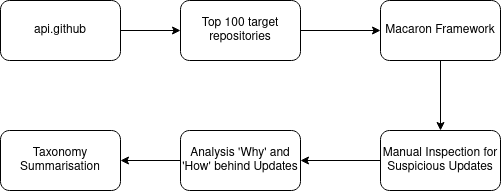
\includegraphics[width=0.7\textwidth]{./screenshot/research_flow.png}
\end{center}


\subsection{Research Aims}
This research is aim to contribute the Macaron framework, then examine top 100 Python and Java Git 
repositories with this framework. The statistical findings will be further concluded through the further process.
Also, the results will provide the developers and maintainers with a good understanding 
of the vulnerabilities existed in their CI/CD pipelines configuration. Furthermore, the reason behind
these unsafe update will be deeply investigated.

\subsection{Research Objectives}
\begin{enumerate}
    \item First step: Fetch the repositories build from Python and Java with the top 100 most stars.
    \item Second step: Input the repositories name into the Macaron Framework to analysis. 
    \item Third step: Summarize the outputs generated by Macaron and visualize the results with graphs.
    \item Fourth step: Manually inspecting the code base from the potentially problematic repositories 
    due to not comply with the requirements from the SLSA.
    \item Fifth step: Document and investigate the reason for this suspicious updates.  
\end{enumerate}
